% Basic document settings.
\documentclass[letterpaper]{article}

% Packages.
\usepackage[dvipsnames]{xcolor}
\usepackage[hidelinks]{hyperref}

\usepackage{amsmath}
\usepackage{framed}
\usepackage{listings}
\usepackage{minted}
\usepackage{multicol}
\usepackage{multirow}
\usepackage{stackengine}
\usepackage{tikz}

% No indentation.
\setlength\parindent{0cm}

% Colors.
\definecolor{DarkGreen}{rgb}{0.0,0.6,0.0}

% Listings settings.
\lstset{
    language=C++,
    basicstyle=\ttfamily,
    commentstyle=\color{DarkGreen}\ttfamily,
    showstringspaces=false,
    keywordstyle=\color{blue}\ttfamily,
    stringstyle=\color{red}\ttfamily,
}

% New commands.
\newcommand{\cpp}{\lstinline|c++|}

% Margins and general layout - Vertical variables.
\topmargin=0mm
\headheight=6mm 
\headsep=1.2cm 
\textheight=22.cm 
\footskip=1cm
\linespread{1.0} 
\addtolength{\voffset}{-0.5in}

% Margins and general layout - Horizontal variables.
\oddsidemargin=2.1cm 
\evensidemargin=1.7 cm 
\textwidth=17.0cm
\addtolength{\hoffset}{-1.0in}
\setlength{\parindent}{0cm}

% Title and author.
\title{Stochastic Models}
\author{Andr\'es Garc\'ia Escovar}
\date{\today}

% Begin document.
\begin{document}
    \maketitle
    \tableofcontents
    \newpage
    %%%%%%%%%%%%%%%%%%%%%%%%%%%%%%%%%%%%%%%%%%%%%%%%%%%%%%%%%%%%%%%%%%%%%%%%%%%%
    % System Diagrams - 1D
    %%%%%%%%%%%%%%%%%%%%%%%%%%%%%%%%%%%%%%%%%%%%%%%%%%%%%%%%%%%%%%%%%%%%%%%%%%%%
    \section{System Diagrams - 1D}

    \begin{tikzpicture}[remember picture, overlay] 
        % 1D Ads Des
        % Boxes
        \draw (0,0) rectangle (+4.8333cm,-4.8333cm);
        \draw (+0.1450cm,-1.9333cm) -- (+4.6883cm,-1.9333cm);
        \draw (+0.2900cm,-1.9333cm) -- (+0.2900cm,-1.4939cm);
        \draw (+0.7153cm,-1.9333cm) -- (+0.7153cm,-1.4939cm);
        \draw (+1.1407cm,-1.9333cm) -- (+1.1407cm,-1.4939cm);
        \draw (+1.5660cm,-1.9333cm) -- (+1.5660cm,-1.4939cm);
        \draw (+1.9913cm,-1.9333cm) -- (+1.9913cm,-1.4939cm);
        \draw (+2.4167cm,-1.9333cm) -- (+2.4167cm,-1.4939cm);
        \draw (+2.8420cm,-1.9333cm) -- (+2.8420cm,-1.4939cm);
        \draw (+3.2673cm,-1.9333cm) -- (+3.2673cm,-1.4939cm);
        \draw (+3.6927cm,-1.9333cm) -- (+3.6927cm,-1.4939cm);
        \draw (+4.1180cm,-1.9333cm) -- (+4.1180cm,-1.4939cm);
        \draw (+4.5433cm,-1.9333cm) -- (+4.5433cm,-1.4939cm);
        \fill [black] (+0.7153cm,-1.3006cm) circle (0.1450);
        \fill [black] (+2.4167cm,-1.3006cm) circle (0.1450);
        \fill [black] (+2.8420cm,-1.3006cm) circle (0.1450);
        \fill [black] (+3.2673cm,-1.3006cm) circle (0.1450);
        \fill [black] (+3.6927cm,-1.3006cm) circle (0.1450);
        \fill [black] (+4.1180cm,-1.3006cm) circle (0.1450);
        % Adsorbing particles
        \draw [->] (+1.5660cm,-1.0062cm) -- (+1.5660cm,-1.4456cm);
        \fill [black] (+1.5660cm,-0.8129cm) circle (0.1450);
        % Adsorbing particles
        \draw [->] (+0.7153cm,-1.1073cm) -- (+0.7153cm,-0.6679cm);
        \draw [->] (+2.4167cm,-1.1073cm) -- (+2.4167cm,-0.6679cm);
        \draw [->] (+3.6927cm,-1.1073cm) -- (+3.6927cm,-0.6679cm);
        % Labels
        \node at (+2.4167cm,-4.3500cm) {Adsorption - Desorption};
        \node at (+0.4833cm,-0.4833cm) {\footnotesize{Easy}};
        \node at (+2.4167cm,-0.4833cm) {\footnotesize{Moderate}};
        \node at (+3.6975cm,-0.4833cm) {\footnotesize{Hard}};
        \node at (+1.7642cm,-1.4500cm) {\footnotesize{P}};
        % Other elements
        \draw (+1.2083cm,-3.8667cm) -- (+1.6477cm,-3.8667cm);
        \draw (+1.4280cm,-3.8667cm) -- (+1.4280cm,-3.4273cm);
        
        % Adsorbing particles
        \draw [->] (+1.4280cm,-2.9395cm) -- (+1.4280cm,-3.3789cm);
        \fill [black] (+1.4280cm,-2.7462cm) circle (0.1450);
        
        \draw (+3.6250cm,-3.8667cm) -- (+3.1856cm,-3.8667cm);
        \draw (+3.4053cm,-3.8667cm) -- (+3.4053cm,-3.4273cm);
        \fill [black] (+3.4053cm,-3.2339cm) circle (0.1450);
        
        % Adsorbing particles
        \draw [->] (+3.4053cm,-3.0406cm) -- (+3.4053cm,-2.6012cm);
        \node at (+2.4167cm,-3.4536cm) {\footnotesize{or}};
    \end{tikzpicture}
       
    %%%%%%%%%%%%%%%%%%%%%%%%%%%%%%%%%%%%%%%%%%%%%%%%%%%%%%%%%%%%%%%%%%%%%%%%%%%%
    % System Diagrams - 2D
    %%%%%%%%%%%%%%%%%%%%%%%%%%%%%%%%%%%%%%%%%%%%%%%%%%%%%%%%%%%%%%%%%%%%%%%%%%%%
    \newpage
    \section{System Diagrams - 2D}

    \begin{tikzpicture}[remember picture, overlay]
        
    \end{tikzpicture}

    %%%%%%%%%%%%%%%%%%%%%%%%%%%%%%%%%%%%%%%%%%%%%%%%%%%%%%%%%%%%%%%%%%%%%%%%%%%%
    % Flow Charts for Kinetic Monte Carlo Algorithms
    %%%%%%%%%%%%%%%%%%%%%%%%%%%%%%%%%%%%%%%%%%%%%%%%%%%%%%%%%%%%%%%%%%%%%%%%%%%%
    \newpage
    \section{Flow Charts for Kinetic Monte Carlo Algorithms}

    %%%%%%%%%%%%%%%%%%%%%%%%%%%%%%%%%%%%%%%%%%%%%%%%%%%%%%%%%%%%%%%%%%%%%%%%%%%%
    % Flow Charts for Kinetic Monte Carlo Algorithms - RSA with Nearest 
    % Neighbor Exclusion
    %%%%%%%%%%%%%%%%%%%%%%%%%%%%%%%%%%%%%%%%%%%%%%%%%%%%%%%%%%%%%%%%%%%%%%%%%%%%

    \subsection{RSA with Nearest Neighbor Exclusion}

    We shall consider one-dimensional lattice with $L$ sites. The lattice is
    a periodic lattice, meaning that the first and last sites in the lattice
    are neighbours. The lattice is initially empty, and particles can adsorb
    onto the lattice with a rate $k$. The particles are assumed to be
    hard-core particles, meaning that they cannot occupy the same site.
    Additionally, the particles interact such that they cannot sit next to
    each other on nearest neighbour sites. Once the particles are adsorbed onto
    the lattice, they cannot move and/or desorb.\bigbreak
    Define the quantities:
    \begin{gather*}
        N_{a}\equiv\text{Adsorption attempts},\qquad
        N_{\text{ads}}\equiv\text{Adsorption attempts},\qquad
        N_{\text{ads}} \leq N_{a}\\
        %
        \Theta\leq\frac{N_{\text{ads}}}{L}\equiv\text{Coverage},\qquad
        k\equiv\text{Rate per site},\qquad
        R_{\text{tot}}=kL\equiv\text{Total rate}\\
        %
        t = \frac{1}{k}\frac{N_{a}}{L}\equiv\text{Physical time},\qquad
        \delta = \frac{1}{R_{\text{tot}}}\rightarrow
        \delta = -\frac{\ln\left(x\right)}{R_{\text{tot}}}\equiv
        \text{{Physical time per attempt.}}\\
        x\in\left(0,1\right)
    \end{gather*}
    \underline{Considerations}:
    \begin{itemize}
        \item Sites are chosen at random and the system configuration is updated
        after each successful attempt.
        \item RSA simulations are efficient except for long times where few
        adsorption sites remain $\rightarrow$ most adsorption attempts fail;
        alternative, track adsorption sites.
    \end{itemize} 

    %%%%%%%%%%%%%%%%%%%%%%%%%%%%%%%%%%%%%%%%%%%%%%%%%%%%%%%%%%%%%%%%%%%%%%%%%%%%
    % Flow Charts for Kinetic Monte Carlo Algorithms - Glauber Spin Flip
    % Dynamics
    %%%%%%%%%%%%%%%%%%%%%%%%%%%%%%%%%%%%%%%%%%%%%%%%%%%%%%%%%%%%%%%%%%%%%%%%%%%%

    \subsection{Glauber Spin Flip Dynamics}

    We shall consider a one-dimensional lattice with $L$ sites; where the
    lattice is assumed to be periodic. All the sites are populated with a spin,
    which can be either up ($\uparrow$) or down ($\downarrow$). The spins will
    interact with their nearest neighbours, such that the spins will flip with a
    rate $k$, depending on the state of their spin and that of their neighbor.
    \begin{gather*}
        N_{a}\equiv\text{Spin flip attempts},\qquad
        \omega_j\equiv\text{Spin flip rate for site }j,\\
        %
        \omega_{j}\text{ can take one of three states: }
        \omega_0 = \alpha,\,\,
        \omega_{\pm} = \alpha\left(
        1 \pm \tanh\left(2\beta J\right)
        \right)\,\,\text{and}\,\, \omega_{\text{max}} = 
        \max\left(\omega_{+},\omega_{-}\right)\\
        %
        \omega_{\text{max}}\equiv\text{Maximum rate per site},\quad
        R_{\text{tot}}^{\text{max}}=\omega_{\text{max}}L\equiv
        \text{Total maximum rate.}\\
        %
        t = \frac{1}{\omega_{\text{max}}}
        \frac{N_{a}}{L}\equiv\text{Physical time},\qquad
        \delta = \frac{1}{R_{\text{tot}}^{\text{max}}}\rightarrow
        \delta = -\frac{\ln\left(x\right)}{R_{\text{tot}}^{\text{max}}}\equiv
        \text{{Physical time per attempt.}}\\
        x\in\left(0,1\right)
    \end{gather*}
    \underline{Considerations}:
    \begin{itemize}
        \item Sites are chosen at random and the system configuration is updated
        after each successful attempt.
        \item Glauber simulation is efficient unless $\omega_{+}>>\omega_{0}$
        and $\omega_{+}>>\omega_{-}$, and the system has evolved to large
        clusters of aligned spins.
    \end{itemize}

    %%%%%%%%%%%%%%%%%%%%%%%%%%%%%%%%%%%%%%%%%%%%%%%%%%%%%%%%%%%%%%%%%%%%%%%%%%%%
    % Flow Charts for Kinetic Monte Carlo Algorithms - Irreversible Island 
    % Formation During Deposition
    %%%%%%%%%%%%%%%%%%%%%%%%%%%%%%%%%%%%%%%%%%%%%%%%%%%%%%%%%%%%%%%%%%%%%%%%%%%%

    \subsection{Irreversible Island Formation During Deposition}

    Consider a system in which particles are deposited at a rate $F$ per site.
    Adsorbed atoms with no neighbors hop left and right at a rate $h$. If
    an atom happens to be a neighbor of another atom, it can't hop or desorb.
    
    % Algorithm
    \subsubsection{Algorithm}
    Define:
    \begin{gather*}
        F+2h\equiv\text{Maximum rate per site},\qquad
        R_{\text{tot}}^{\text{max}}=\left(F+2h\right)L\equiv\text{total
        maximum rate.}\\
        %
        \delta = \frac{1}{R_{\text{tot}}^{\text{max}}}\rightarrow
        \delta = -\frac{\ln\left(x\right)}{R_{\text{tot}}^{\text{max}}}\equiv
        \text{{Physical time per attempt.}}\\
        x\in\left(0,1\right)
    \end{gather*}
    \begin{itemize}
        \item Pick a site randomly.
        \item Attempt to deposit a particle with probability
        $q_\text{dep}=F/\left(F+2h\right)$; provided the chosen site
        is empty.
        \item Attempt to hop with probability
        $q_\text{dep}=2h/\left(F+2h\right)$; provided the chosen site
        contains a particle and does not have any neighbors.
        \begin{enumerate}
            \item If there are no neighbors, hop with probability 
            $h$ to either site.
        \end{enumerate}
    \end{itemize}
    This algorithm can be very inneficient because the typical ratio
    $h/F$ is in the range $10^{6} - 10^{19}$ $\rightarrow$ mainly attempt to
    hop, but density of active isolated particles is too low.
    \begin{center}
        \fbox{\begin{minipage}{5cm}
            \begin{center}
                \underline{Alternative}:
                \textquotedblleft Bortz Algorithm\textquotedblright
            \end{center}
        \end{minipage}}
    \end{center}

    % Bortz Algorithm
    \subsubsection{Algorithm}
    
    Tracks only the active isolated particles. Define:
    \begin{gather*}
        N_{h}\equiv\text{Numer of isolated particles},\\
        %
        R_{text{dep}}=FL\equiv\text{Maximum total deposition rate},\qquad
        R_{text{hop}}=2h\cdot N_{h}\equiv\text{Total hop rate},\\
        %
        P_{\text{dep}} = \frac{R_{\text{dep}}}{R_{\text{dep}}+R_{\text{hop}}}
        \equiv{\text{Deposition probability}},
        \quad
        P_{\text{hop}} = \frac{R_{\text{hop}}}{R_{\text{dep}}+R_{\text{hop}}}
        \equiv{\text{Hopping probability}}.
    \end{gather*}
\end{document}